% !TeX root = main.tex

\subsection{Assignment 1: Motion planning using RRT}

\subsubsection*{RRT Algorithm}

The RRT algorithm has the following steps

\begin{enumerate}
    \item \textbf{Define map}, free space, and the problem: This will be a map having the start, stop and the free space information of the environment (including a list of obstacles).
    \item Keep \textbf{sampling} in free space. Store nodes in a tree (can be modeled as a list with links). Each node in the list has $x, y$, a parent (index), children (indices), and a $v, \omega$ command (to reach it from the parent). We start at the starting point, with zero commands and NULL parent.
    \item When a new point in free space is sampled, the closest point from the nearest node (in the tree) and in the allowed distance is obtained. The control commands to this point is obtained. The node is added (as a child and to the list) if the path from the nearest node to this node is free of collisions.
    \item We repeat the above step will the most recently added node (at the bottom of list) is within a certain bounds of the goal.
\end{enumerate}

The following implementations were done

\begin{itemize}
    \item Generating a path assuming that a holonomic robot is going to travel it (do not store $v, \omega$), and then make a non-holonomic robot travel the path. The robot will either go straight or turn at nodes.
    
    This does not exploit the non-holonomic structure of the vehicle and may not be practical for larger robots. See figure \ref{fig:rrt-holo} for results using this method.

    \item Exploiting the non-holonomic structure of the vehicle when adding nodes. This has the advantage of creating paths and routes that can inherently be traversed by the vehicle.
    
    This involves either directly sampling in the vehicle's control space or running inverse kinematics on the points sampled in the state space (free map). See figure \ref{fig:rrt-nonholo} for results using this method.
\end{itemize}

\begin{figure}[ht]
    \centering
    \begin{subfigure}[b]{0.3\textwidth}
        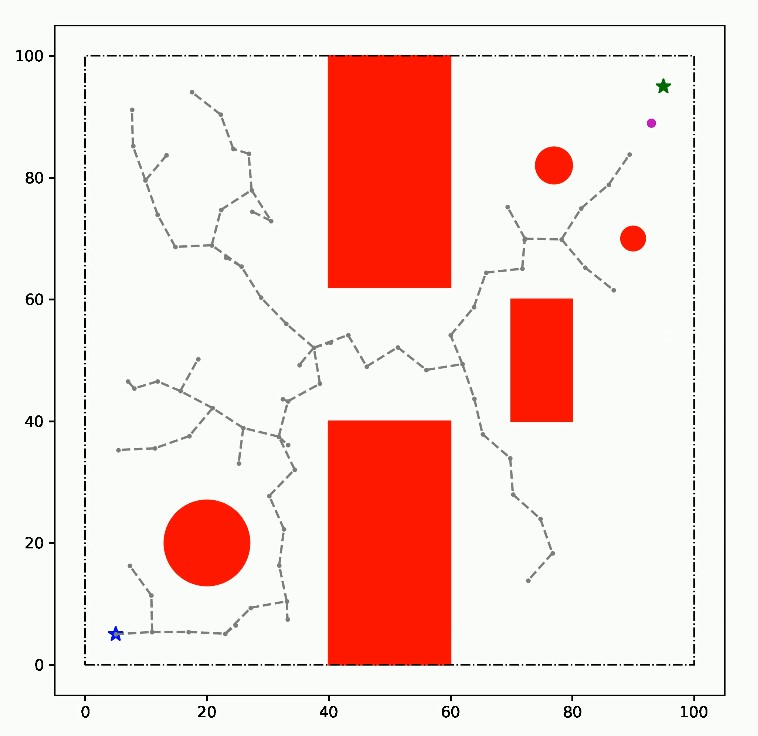
\includegraphics[width=\textwidth]{rrt-holon-sampling.jpg}
        \caption{Sampling}
    \end{subfigure}
    \begin{subfigure}[b]{0.3\textwidth}
        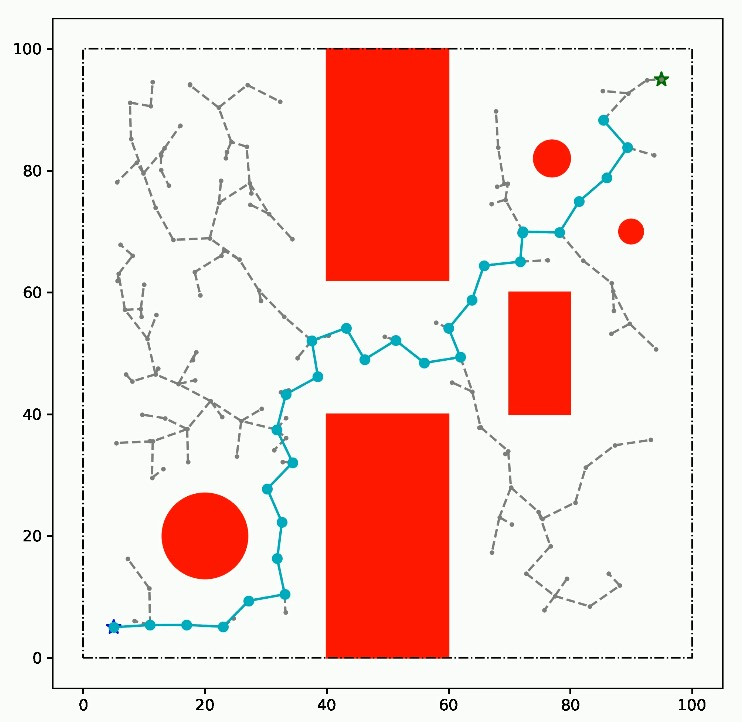
\includegraphics[width=\textwidth]{rrt-holon-path.jpg}
        \caption{Path}
    \end{subfigure}
    \begin{subfigure}[b]{0.3\textwidth}
        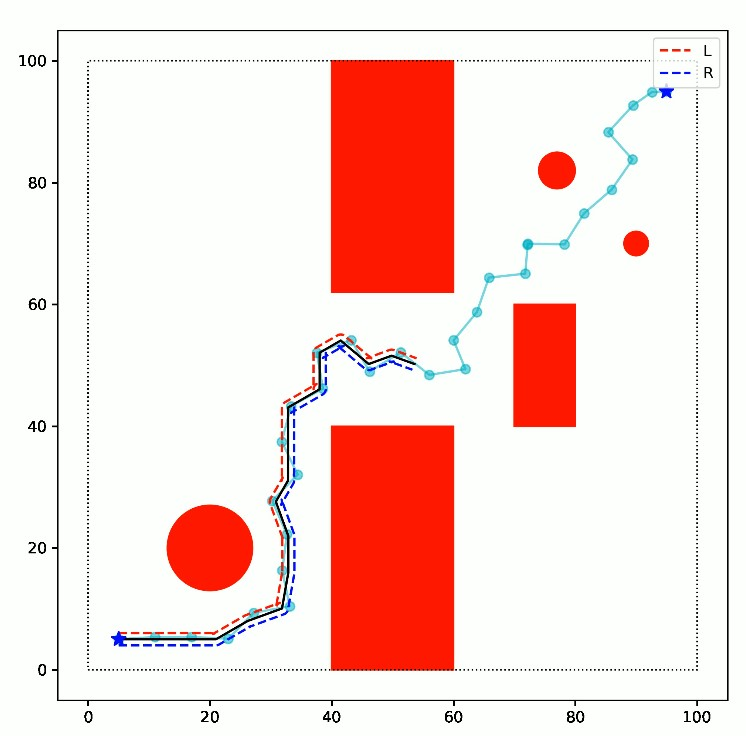
\includegraphics[width=\textwidth]{rrt-holon-nhv.jpg}
        \caption{Traveling}
    \end{subfigure}
    \caption{RRT: Holonomic sampling and non-holonomic travel}
    \label{fig:rrt-holo}
    \small
        The sampling and path are that of a holonomic model. The non-holonomic robot navigates this using a sequence of straight line travels and turning commands.
\end{figure}

\begin{figure}[ht]
    \centering
    \begin{subfigure}[b]{0.3\textwidth}
        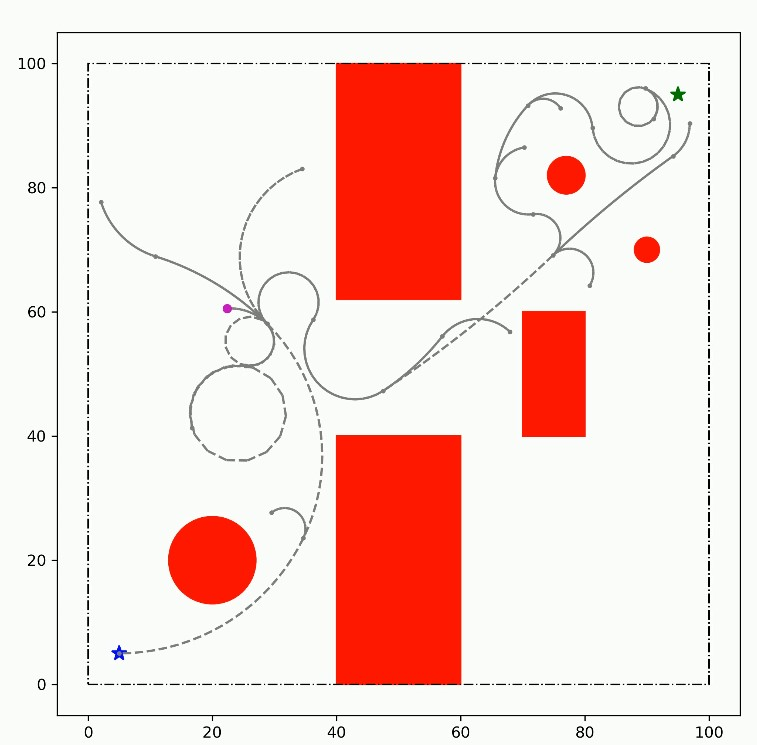
\includegraphics[width=\textwidth]{rrt-nonholon-sampling.jpg}
        \caption{Sampling}
    \end{subfigure}
    \begin{subfigure}[b]{0.3\textwidth}
        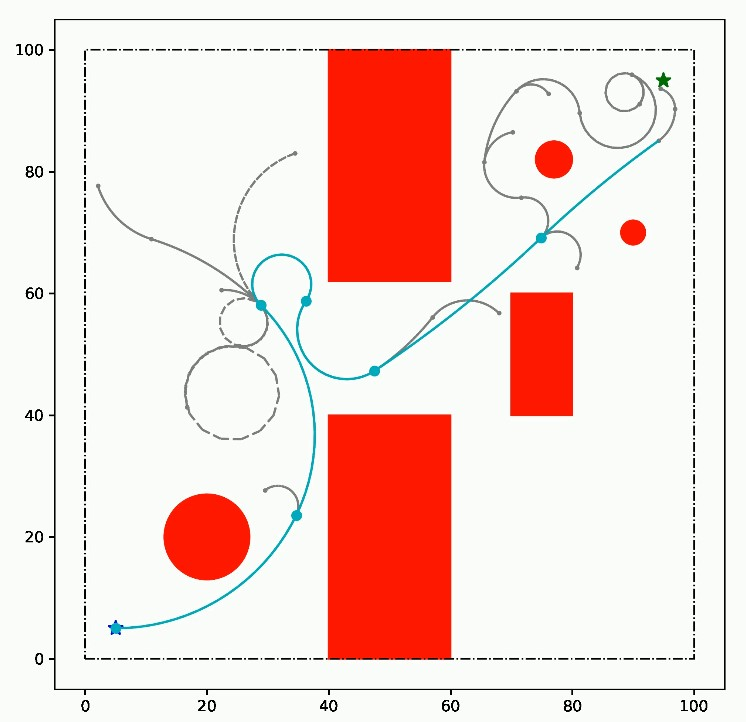
\includegraphics[width=\textwidth]{rrt-nonholon-path.jpg}
        \caption{Path}
    \end{subfigure}
    \begin{subfigure}[b]{0.3\textwidth}
        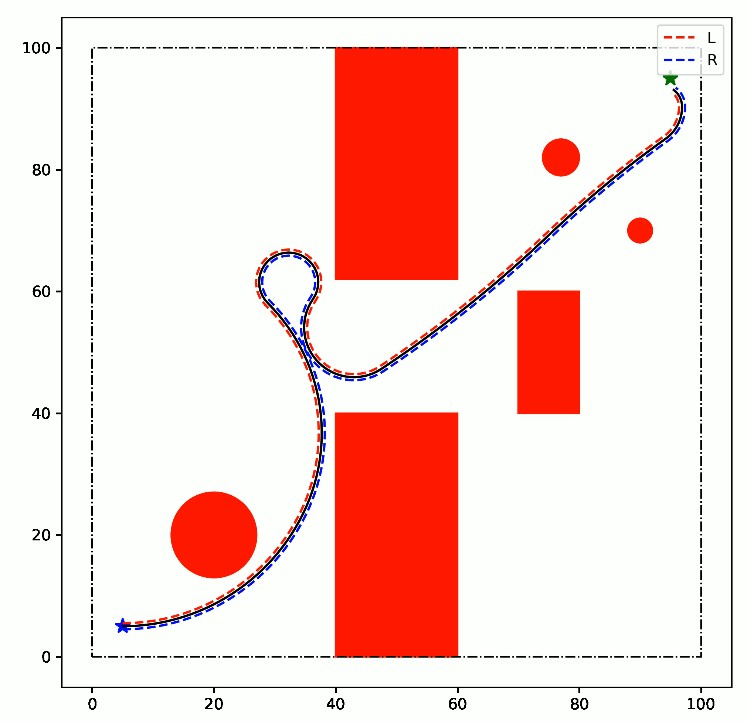
\includegraphics[width=\textwidth]{rrt-nonholon-veh.jpg}
        \caption{Traveling}
    \end{subfigure}
    \caption{RRT: Non-holonomic sampling and travel}
    \label{fig:rrt-nonholo}
    \small
        The sampling, path generation and traveling is of a differential drive robot (non-holonomic robot).
\end{figure}
